\documentclass{article}
\usepackage{graphicx}
\usepackage{enumerate}
\usepackage[margin=1in]{geometry}
\graphicspath{ {images/} }
\begin{document}

\section {Caputing a bulk TCP transfer from your computer to a remote server answers}
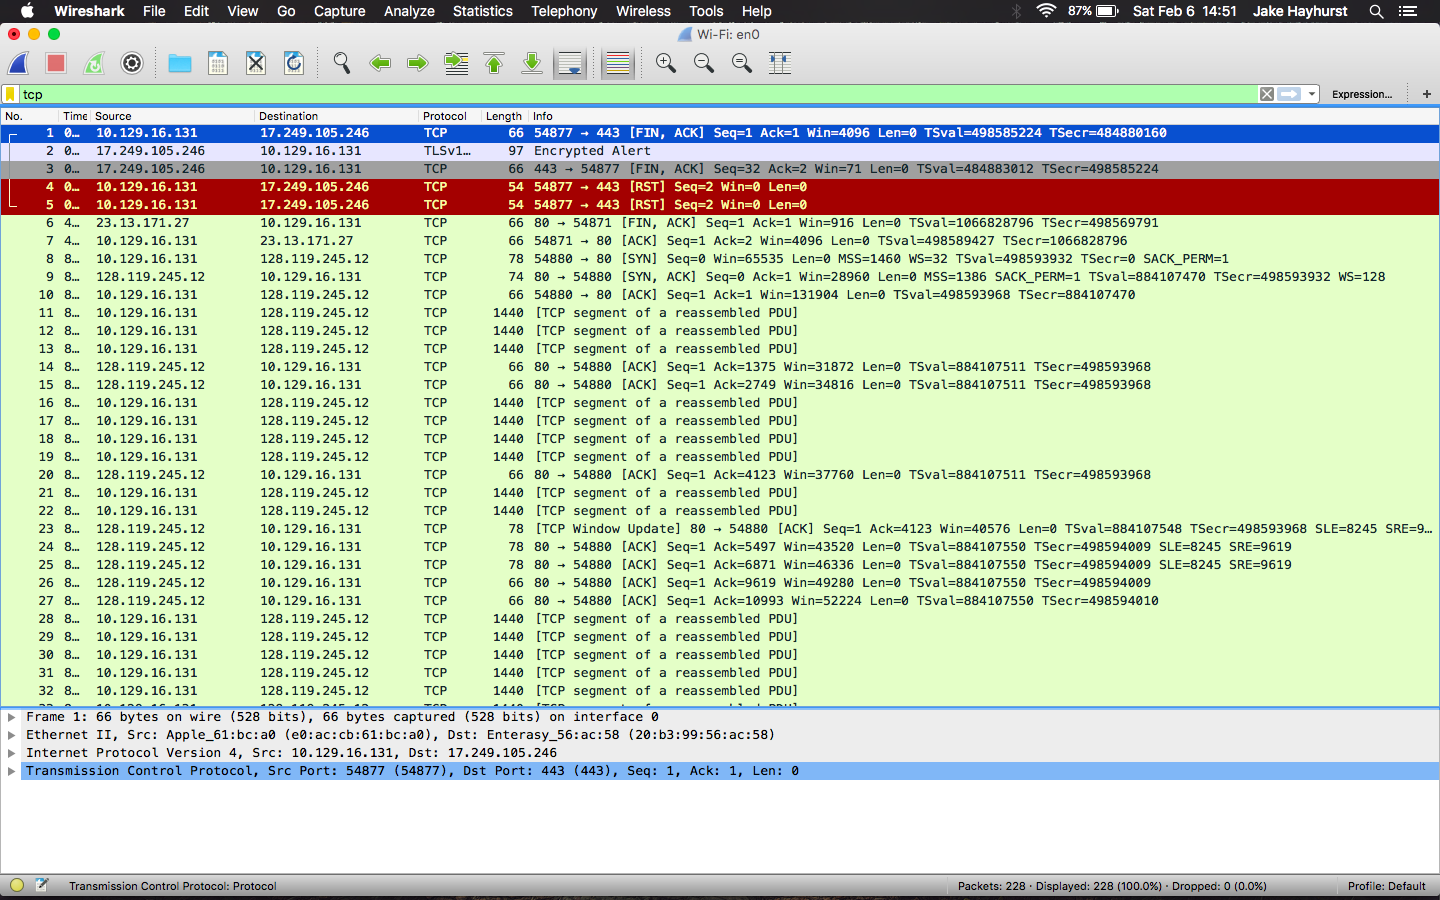
\includegraphics[width=\textwidth]{part1TCP}\\\\

\section {A first look at the captured trace}
\begin{itemize}
  \item The IP address from the source is 192.168.1.102 and the TCP port number being used by the source is 1161
  \item The IP address from the server is 128.119.245.12 and the TCP port number being used by the source is 80
  \item My IP address is 10.129.16.131 and the TCP port number being used is 54877
\end{itemize}

\section {TCP Basics}
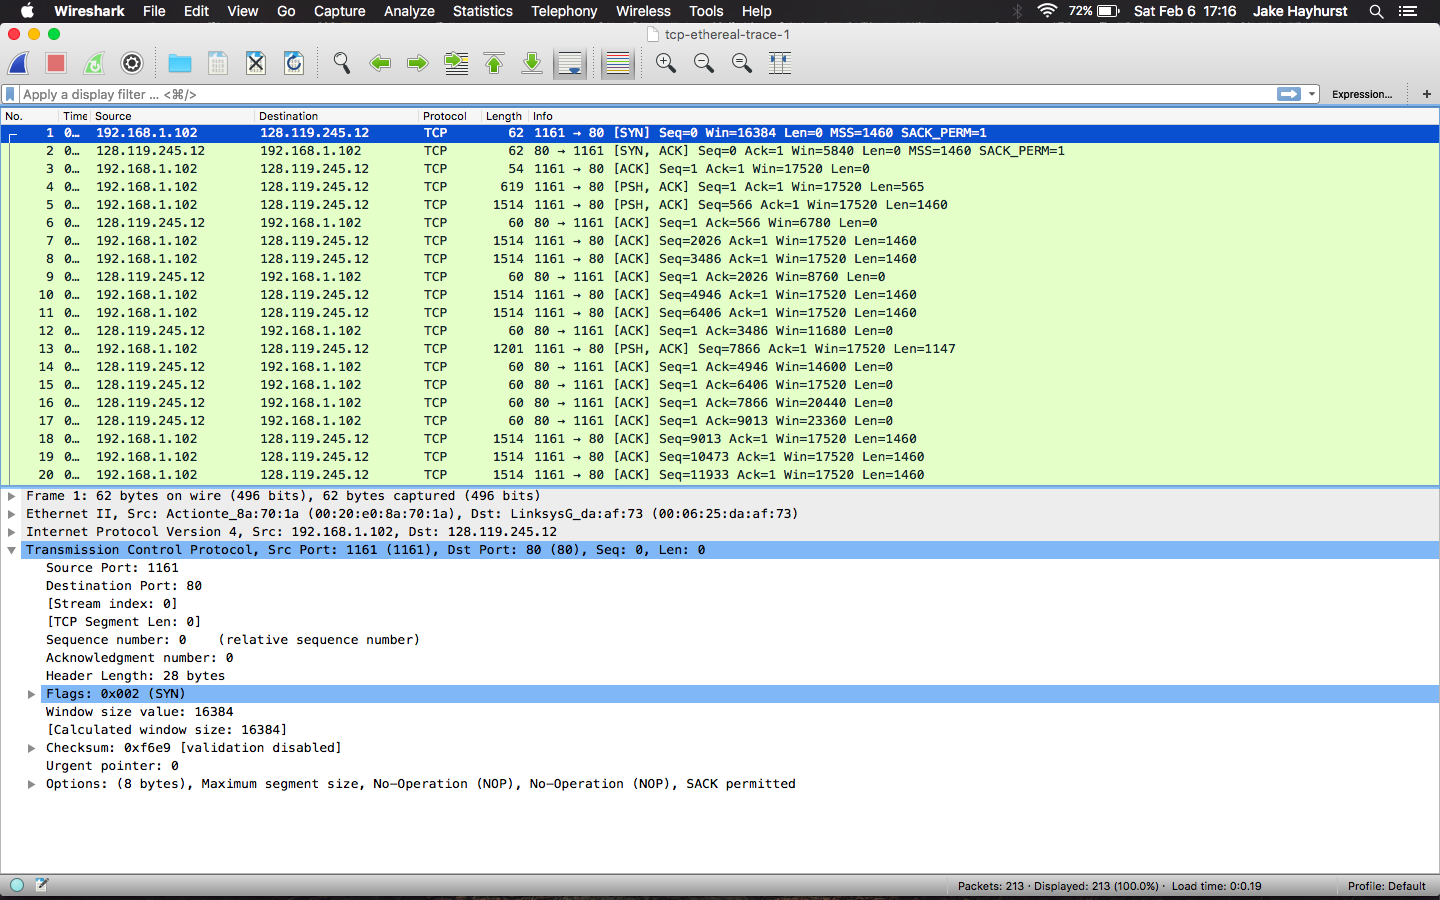
\includegraphics[width=\textwidth]{part3SYN}\\\\
\begin{itemize}
  \item The sequence number of the TCP SYN segment that is used to initiate the TCP connection is 0.
  \item The sequence number of the SYNACK segment sent by the server in reply was 0, the value of the acknowledgement field is 1. This value is determined by the server adding 1 to the sequence so that the server can indicate to the client that the next segment should be, in this case, 1.
  \item The sequence number of the TCP segment containing the HTTP POST command is 1 and is located on frame 4.
  \item The with the HTTP POST segment is considered as the first segment. Segments 1 to 6 are frame numbers 4, 5, 7, 8, 10, 11; the acknowledgements are on frames 6, 9, 12, 14, 15, 16.\\
  \begin{tabular}{||c c c c||}
    \hline
     & Sent Time & ACK received time & RTT \\ [0.5ex]
    \hline\hline
    1 & 0.026477 & 0.053937 & 0.02746 \\
    \hline
    2 & 0.041737 & 0.077294 & 0.035557 \\
    \hline
    3 & 0.054026 & 0.124085 & 0.070059 \\
    \hline
    4 & 0.054690 & 0.169118 & 0.11443 \\
    \hline
    5 & 0.077405 & 0.217299 & 0.13989 \\
    \hline
    6 & 0.078157 & 0.267802 & 0.18964\\
    \hline
  \end{tabular}\\\\
  $Estimated RTT = (1 - \alpha) * EstimatedRTT + \alpha * SampleRTT$
  EstimatedRTT after the receipt of the ACK of 1\\
  $Estimated RTT = RTT for 1 = 0.02746$\\\\
  EstimatedRTT after the receipt of the ACK of 2\\
  $Estimated RTT = 0.875 * 0.02746 + 0.125 * 0.035557 = 0.0285$\\\\
  EstimatedRTT after the receipt of the ACK of 3\\
  $Estimated RTT = 0.875 * 0.0285 + 0.125 * 0.070059 = 0.0337$\\\\
  EstimatedRTT after the receipt of the ACK of 4\\
  $Estimated RTT = 0.875 * 0.0337 + 0.125 * 0.11443 = 0.0438$\\\\
  EstimatedRTT after the receipt of the ACK of 5\\
  $Estimated RTT = 0.875 * 0.0438 + 0.125 * 0.13989 = 0.0558$\\\\
  EstimatedRTT after the receipt of the ACK of 6\\
  $Estimated RTT = 0.875 * 0.0558 + 0.125 * 0.18964 = 0.0725$\\
  \item The length of the first TCP segment is 465 bytes the rest of the TCP segments are 1460 bytes
  \item The minimum amount of buffer space advertised for the sender is 5840. The sender is never throttled due to lacking of receiving buffer space.
  \item There are no retransmitted segments in the trace, this can be seen by the Time Sequence Graph (stephens)
  \item The receiver typically acknowledges roughly 1460 bytes in an ACK.The difference between the acknowledged sequences by two consecutive ACKs show that the data received by the server between the two ACKs. There are cases where the receiver is ACKing every other segment. An example of this is frame 80 where the server ACKs twice as much as the previous ACK
  \item The way to calculate the throughput (bytes transferred per unit time) for the TCP connection is:\\
  $(Last ACK - 1) / (End of Transmission Time - Start of Transmission Time)$\\
  In this case our solution is:\\
  $(164091 -1) / (5.455830 - 0.026477) = 164090 / 5.4294 = 30.222 $KBytes/sec\\
  I do this because the last ACK minus 1 will give us the total data transmitted with the total
\end{itemize}

\section {TCP congestion control in action}
\begin{itemize}
  \item Slow start begins the connection, the congestion avoidance phase is dependent on the congestion window size of the TCP sender. The value of the congestion window size cannot be obtained from the Time Sequence Graph.
  \item The ideal behavior of TCP is that the slow start will stop congestion from happening off the bat and will then will activate congestion control if too many packets are lost. For this connection we send some small objects that are finished transmitting before slow start is over causing a delay because of the slow start phase.  
\end{itemize}

\end{document}
